\documentclass{standalone}

\usepackage{amssymb}
\usepackage{amsthm}
\usepackage{amsmath}


\usepackage{tikz}
\usetikzlibrary{shapes,backgrounds,calc,patterns}
\usepackage{venndiagram}


\begin{document}
    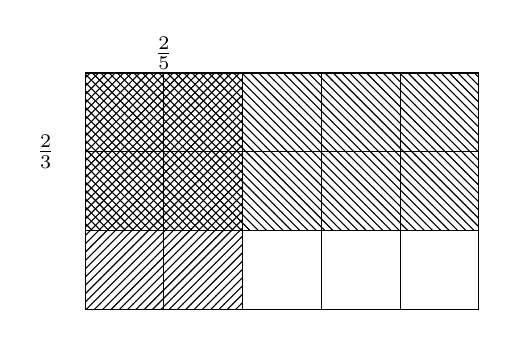
\begin{tikzpicture}
\draw (0,0) rectangle (5,3);
\draw (1,0) -- (1,3);
\draw (2,0) -- (2,3);
\draw (3,0) -- (3,3);
\draw (4,0) -- (4,3);
\draw (0,1) -- (5,1);
\draw (0,2) -- (5,2);
\pattern[pattern=north east lines] (0,0) rectangle (2,3);
\node at (1,3.25) {\(\frac{2}{5}\)};
\pattern[pattern=north west lines] (0,3) rectangle (5,1);
\node at (-.5,2) {\(\frac{2}{3}\)};
\end{tikzpicture}
\end{document}